%%%%%%%%%%%%%%%%%%%%%%%%%%%%%%%%%%%%%%%%%%%%%%%%%%%%%%%%%%%%%%%%%%%%%%%%%%%%%%%
%
% Tommy P. Keane
% Master of Science Thesis
% Department of Electrical and Microelectronic Engineering
% Rochester Institute of Technology
%
% Presented: May 12, 2011
%
%%%%%%%%%%%%%%%%%%%%%%%%%%%%%%%%%%%%%%%%%%%%%%%%%%%%%%%%%%%%%%%%%%%%%%%%%%%%%%%
\documentclass[serif]{beamer}

\setbeamertemplate{caption}[numbered]

\usepackage{amsmath}
\usepackage{amssymb}
\usepackage{xfrac}
\usepackage{graphicx}
\graphicspath{{./images}}
\usepackage{subfigure}
\usepackage{color}

\usepackage[center]{caption}

\usepackage{concrete}

\bibliographystyle{unsrt}

\usetheme{Warsaw}


%%%%%%%%%%%%%%%%%%%%%%%%%%%%%%%%%%%%%%%%%%%%%%%%%%%%%%%%%%%%%%%%%%%%%%%%%%%%%%%
% FRONT MATTER
%%%%%%%%%%%%%%%%%%%%%%%%%%%%%%%%%%%%%%%%%%%%%%%%%%%%%%%%%%%%%%%%%%%%%%%%%%%%%%%
\title[M.S. Thesis: WFMI\hspace{10em}\insertframenumber{ }of \inserttotalframenumber]{\large\textsc{Weighted and Filtered Mutual Information}:
   \\
   A metric for automated creation of panoramas\\from views of complex scenes}
\author{Tommy P. Keane}
\institute{Thesis Defense Presentation \\ \vskip .1in Partial Fulfillment of the Degree of Master of Science \\ \vskip .1in Department of Electrical and Microelectronic Engineering \\ Rochester Institute of Technology \\ Rochester, NY 14623 \\ \vskip .1in Presented on:}
\date{\vskip -.2in May 12, 2011}


%%%%%%%%%%%%%%%%%%%%%%%%%%%%%%%%%%%%%%%%%%%%%%%%%%%%%%%%%%%%%%%%%%%%%%%%%%%%%%%
% BEGIN DOCUMENT
%%%%%%%%%%%%%%%%%%%%%%%%%%%%%%%%%%%%%%%%%%%%%%%%%%%%%%%%%%%%%%%%%%%%%%%%%%%%%%%
\begin{document}

%%%%%%%%%%%%%%%%%%%%%%%%%%%%%%%%%%%%%%%%%%%%%%%%%%%%%%%%%%%%%%%%%%%%%%%%%%%%%%%
% TITLE SLIDE
\begin{frame}
\titlepage
\end{frame}



%%%%%%%%%%%%%%%%%%%%%%%%%%%%%%%%%%%%%%%%%%%%%%%%%%%%%%%%%%%%%%%%%%%%%%%%%%%%%%%
% ABSTRACT
%\begin{frame}[c]{Abstract}
%\noindent
%%%%%%%%%%%%%%%%%%%%%%%%%%%%%%%%%%%%%%%%%%%%%%%%%%%%%%%%%%%%%%%%%%%%%%%%%%%%%%%%%
%
% Tommy P. Keane
% Master of Science Thesis
% Department of Electrical and Microelectronic Engineering
%
% March 2011
%
%
%
%%%%%%%%%%%%%%%%%%%%%%%%%%%%%%%%%%%%%%%%%%%%%%%%%%%%%%%%%%%%%%%%%%%%%%%%%%%%%%%

%%%%%%%%%%%%%%%%%%%%%%%%%%%%%%%%%%%%%%%%%%%%%%%%%%%%%%%%%%%%%%%%%%%%%%%%%%%%%%%
%
% ABSTRACT
%
%%%%%%%%%%%%%%%%%%%%%%%%%%%%%%%%%%%%%%%%%%%%%%%%%%%%%%%%%%%%%%%%%%%%%%%%%%%%%%%


%%%%%%%%%%%%%%%%%%%%%%%%%%%%%%%%%%%%%%%%%%%%%%%%%%%%%%%%%%%%%%%%%%%%%%%%%%%%%%%
% BEGIN DOCUMENT
\begin{doublespace}

To contribute a novel approach in the field of image registration and panorama creation, this algorithm foregoes any scene knowledge, requiring only modest scene overlap and an acceptable amount of entropy within each overlapping view, both empirically derived. The weighted and filtered mutual information (WFMI) algorithm has been developed for stationary, color, surveillance video cameras and relies on color gradients for feature correspondence. This is a novel extension of well-established maximization of mutual information (MMI) algorithms. Where MMI algorithms are typically applied to high altitude photography and medical imaging (scenes with relatively simple shapes and affine homographies between views), the WFMI algorithm has been designed for scenes with occluded objects and significant parallax. Despite the typically non-affine surveillance scenarios, searching in the affine space is a practical assumption that provides computational efficiency and accurate results, even with complex scene views that suffer from parallax and occlusions. The WFMI algorithm can perfectly register affine views, performs exceptionally well with near-affine related views, and in complex (projective) views with parallax and occlusion the WFMI algorithm provides an accurate estimate of the overlap regions between the views. The WFMI algorithm uses simple calculations (vector field gradient, Laplacian filtering, and feature histograms) to generate the WFMI metric and provide the optimal affine relationship. This algorithm is unique when compared to typical MMI algorithms and modern registration algorithms because it avoids a lot of \textit{a priori} knowledge and calculations, while still providing an accurate or useful estimate for realistic scenes. With pixel based weightings and the Laplacian filtering operation, the WFMI algorithm overcomes the failures of typical MMI algorithms in scenes where complex or occluded shapes do not provide sufficiently large peaks in the mutual information maps. This work has currently been applied to individual video frames and future work could extend the algorithm into utilizing motion information or temporal frame registrations to enhance scenes with smaller overlap regions, lower entropy, or significant parallax and occlusions.

\end{doublespace}

%%%%%%%%%%%%%%%%%%%%%%%%%%%%%%%%%%%%%%%%%%%%%%%%%%%%%%%%%%%%%%%%%%%%%%%%%%%%%%%
% END OF DOCUMENT

%{\tiny This algorithm performs automatic registration by foregoing any scene knowledge, requiring only modest scene overlap and an acceptable amount of entropy within each overlapping view. The weighted and filtered mutual information (WFMI) algorithm has been developed for stationary, color, surveillance video cameras. This is a novel extension of maximization of mutual information (MMI) algorithms, which are typically applied to scenes with simple shapes and near-affine relationships between views. The WFMI algorithm has been designed for realistic, complex scenes with occlusion and parallax variations between the views. And despite the typically non-affine related surveillance scenarios, the WFMI algorithm is searching only in the affine space for computational efficiency. The WFMI algorithm can perfectly register affine views, performs exceptionally well with near-affine related views, and in complex (projective or polynomial related) views the WFMI algorithm provides an accurate estimate of the overlap region between the views. The WFMI algorithm uses simple calculations (vector field gradient, Laplacian filtering, and feature histograms) to generate the WFMI metric and provide the optimal affine relationship. This work has been applied to individual video frames and future work could extend the algorithm into utilizing motion information or temporal frame registrations to enhance the results.}
%\end{frame}

%\textsc{Reference}:
%\\
%{\tiny T. Keane, E. Saber, H. Rhody, A. Savakis, J. Raj, ''Unsupervised automated panorama creation for realistic surveillance scenes through weighted mutual information registration'', \textit{Proceedings of SPIE/IS\&T: Electronic Imaging Symposium}, San Francisco, CA, Jan. 2011}




%%%%%%%%%%%%%%%%%%%%%%%%%%%%%%%%%%%%%%%%%%%%%%%%%%%%%%%%%%%%%%%%%%%%%%%%%%%%%%%
% WHAT IS THE PROBLEM?
\begin{frame}[c]{\sc What is the Problem?}

\begin{center}

\begin{figure}[!h]
\centering
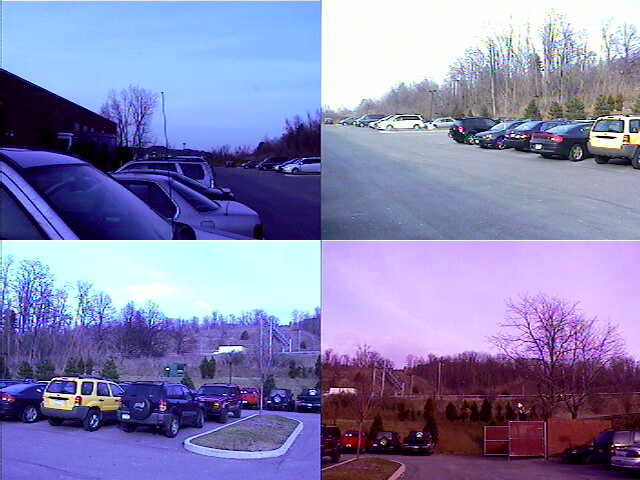
\includegraphics[width=.8\columnwidth]{LenelExample}
\caption{Lenel Parking Lot Example}
\label{LenelExample}
\end{figure}

\end{center}

\end{frame}



%%%%%%%%%%%%%%%%%%%%%%%%%%%%%%%%%%%%%%%%%%%%%%%%%%%%%%%%%%%%%%%%%%%%%%%%%%%%%%%
% WHAT IS AVAILABLE?
\begin{frame}[t]{\sc What is available?}

\begin{center}

\begin{figure}[!h]
\centering
\vfill
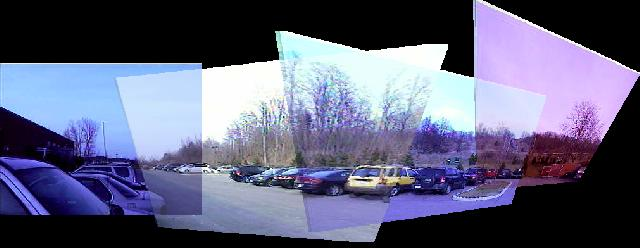
\includegraphics[width=1\columnwidth]{LenelExampleStitched}
\caption{Manually Registered Images from Previous Figure}
\label{LenelExampleStitched}
\end{figure}

\end{center}

\end{frame}



%%%%%%%%%%%%%%%%%%%%%%%%%%%%%%%%%%%%%%%%%%%%%%%%%%%%%%%%%%%%%%%%%%%%%%%%%%%%%%%
% WHAT WAS OUR TASK?
\begin{frame}[c]{\sc What was our task?}

\begin{center}
{\sc Proposed}:
\\
Create an automated algorithm for registering, stitching, and blending the views from stationary color surveillance cameras.
\end{center}

\end{frame}


%%%%%%%%%%%%%%%%%%%%%%%%%%%%%%%%%%%%%%%%%%%%%%%%%%%%%%%%%%%%%%%%%%%%%%%%%%%%%%%
% WHAT HAS BEEN ACHIEVED?
\begin{frame}[t]{\sc What has been achieved?}

\vfill
\begin{center}
{\sc Weighted and Filtered Mutual Information (WFMI)}:
\\
A novel application of mutual information as a metric for determining overlapping portions of unconstrained views of complex, realistic scenes.
\\
\vskip .25in
Implementation in MATLAB\textsuperscript{\textregistered}, C++ with OpenCV
\\
\vskip .25in
Intellectual Property held by \\ Lenel Systems Inc., A UTC Fire and Security Corporation.
\end{center}

\end{frame}


%%%%%%%%%%%%%%%%%%%%%%%%%%%%%%%%%%%%%%%%%%%%%%%%%%%%%%%%%%%%%%%%%%%%%%%%%%%%%%%
% WHY A NEW ALGORITHM?
\begin{frame}[c]{\sc Why a New Algorithm?}
\centering
\textsc{Point-to-Point Correspondences}
\begin{itemize}
\item SIFT
\item Harris Detector
\item FAST Detector
\item SUSAN Detector
\item \textit{et cetera}
\end{itemize}

\begin{block}{\sc Major Concerns}
A new intellectual property (IP) that is robust for extremely general case, can be applied to their existing systems efficiently and quickly, with the intentions of a relatively simple advancement to real-time operation.
\end{block}

\end{frame}




%%%%%%%%%%%%%%%%%%%%%%%%%%%%%%%%%%%%%%%%%%%%%%%%%%%%%%%%%%%%%%%%%%%%%%%%%%%%%%%
% WHAT IS BEING PRESENTED?
\begin{frame}[t]{\sc What is being presented?}

\vfill

\begin{description}
\item[Multiple View Geometry] \hspace*{\fill} \\
System description and constraints.

\item[Mutual Information] \hspace*{\fill} \\
The how and why of the applied theory.

\item[Image Features] \hspace*{\fill} \\
What are they and how are they chosen?

\item[The Proposed Algorithm] \hspace*{\fill} \\
The design and implementation.

\item[Results and Constraints] \hspace*{\fill} \\
Synthetic and real-world examples and achievements.
\end{description}

\end{frame}




%%%%%%%%%%%%%%%%%%%%%%%%%%%%%%%%%%%%%%%%%%%%%%%%%%%%%%%%%%%%%%%%%%%%%%%%%%%%%%%
% TERMINOLOGY
\begin{frame}[c]{\sc Terminology and System Diagram}

\begin{figure}
\centering
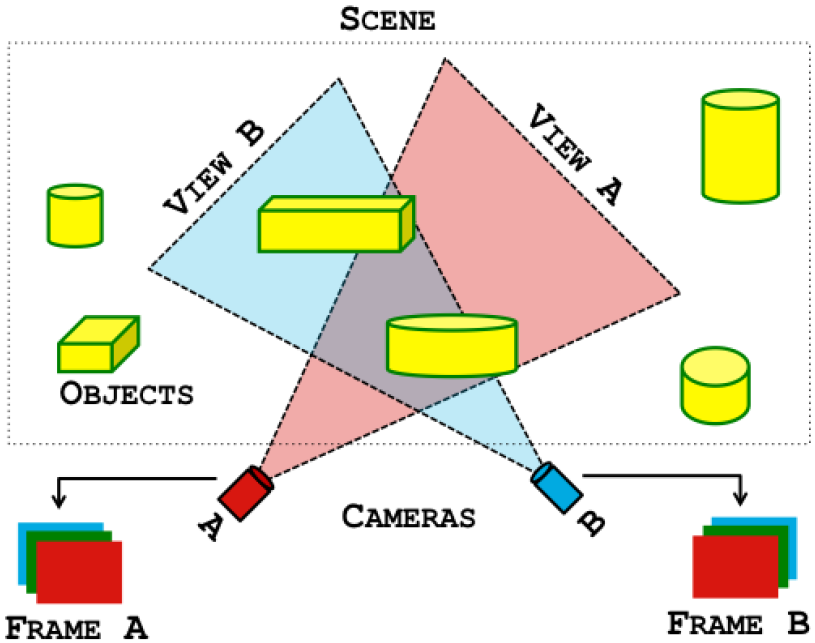
\includegraphics[width=.9\columnwidth]{Terminology}
\label{terminology}
\end{figure}

\end{frame}



%%%%%%%%%%%%%%%%%%%%%%%%%%%%%%%%%%%%%%%%%%%%%%%%%%%%%%%%%%%%%%%%%%%%%%%%%%%%%%%
% SINGLE CAMERA
\begin{frame}[c]{\sc Camera Terminology}

\begin{figure}
\centering
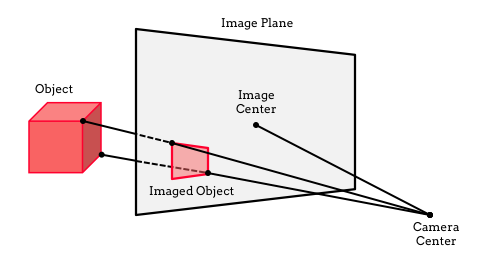
\includegraphics[width=.9\columnwidth]{CameraModel}
\label{SingleCamera}
\end{figure}

\vskip -.1in

\begin{block}{RGB Image Size Notation}
\begin{equation}
\text{Size: }\mathfrak{m} \times \mathfrak{n} \times \mathfrak{p}  \quad \quad \text{Ranges: } [1,\mathfrak{m}], [1,\mathfrak{n}], [1,\mathfrak{p}] \in \mathbb{Z} \nonumber
\end{equation}
\end{block}

\end{frame}


%%%%%%%%%%%%%%%%%%%%%%%%%%%%%%%%%%%%%%%%%%%%%%%%%%%%%%%%%%%%%%%%%%%%%%%%%%%%%%%
% CAMERA CONCERNS
\begin{frame}[c]{\sc Multi-view Concerns}

\begin{figure}
\centering
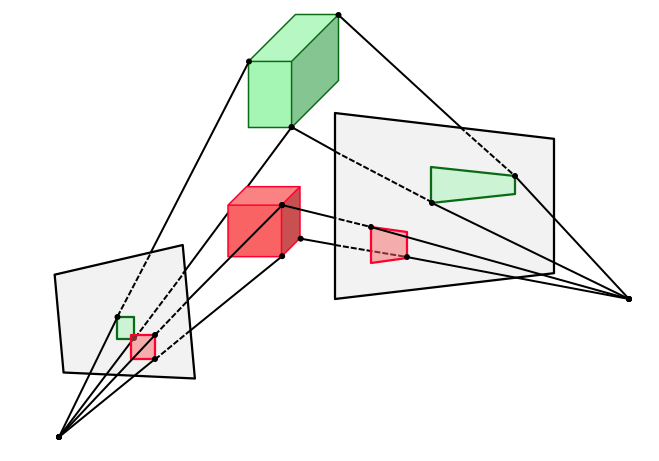
\includegraphics[width=.9\columnwidth]{CameraOcclusion}
\label{TwoCameras}
\end{figure}

\end{frame}


%%%%%%%%%%%%%%%%%%%%%%%%%%%%%%%%%%%%%%%%%%%%%%%%%%%%%%%%%%%%%%%%%%%%%%%%%%%%%%%
% UNDERSTANDING PRACTICAL CONCERNS
\begin{frame}[c]{\sc Understanding Practical Concerns}


\begin{block}<1->{Parallax Disparity}
Angle and distance to objects modifies their size and position in the view.
\end{block}

\vfill

\begin{block}<2->{Occlusion Disparity}
Based on Parallax disparity; concerns data that is lost between views, \textit{i.e.} objects ``covering'' other objects or ``leaving'' the view.
\end{block}


\vfill

\begin{block}<3->{Camera Positions}
Limits overlap amount, large-angle rotations modify view of scene content, and position related to scene content modifies Parallax and Occlusion disparities.
\end{block}

\end{frame}


%%%%%%%%%%%%%%%%%%%%%%%%%%%%%%%%%%%%%%%%%%%%%%%%%%%%%%%%%%%%%%%%%%%%%%%%%%%%%%%
% SYSTEM CONCERNS AND CONSTRAINTS
\begin{frame}[t]{\sc System Concerns and Constraints}

\begin{block}{Multiple View Geometry}
Parallax Disparity and Occlusion Disparity arise from Camera Positions and Scene Content, Structure, and Environmental Conditions
\end{block}

\end{frame}


%%%%%%%%%%%%%%%%%%%%%%%%%%%%%%%%%%%%%%%%%%%%%%%%%%%%%%%%%%%%%%%%%%%%%%%%%%%%%%%
% FIRST ASSUMPTION
\begin{frame}[c]{\sc First Assumption}

\begin{figure}
\centering
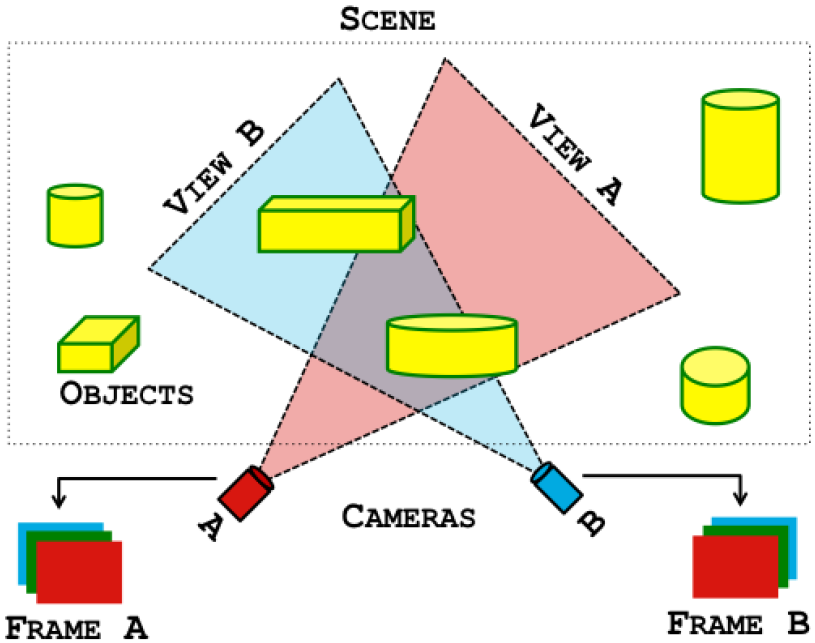
\includegraphics[width=.9\columnwidth]{Terminology}
\label{assumption}
\end{figure}

\end{frame}


%%%%%%%%%%%%%%%%%%%%%%%%%%%%%%%%%%%%%%%%%%%%%%%%%%%%%%%%%%%%%%%%%%%%%%%%%%%%%%%
% DESCRIBING IMAGE DATA
\begin{frame}[c]{\sc Describing Image Data}

\begin{figure}
\centering
\subfigure{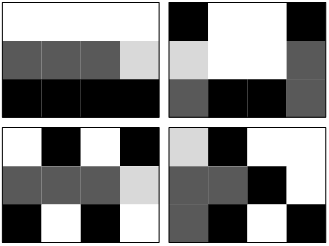
\includegraphics[width=.48\columnwidth]{sampleImages}}
\pause
\subfigure{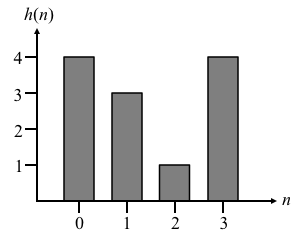
\includegraphics[width=.48\columnwidth]{sampleHistogram}}
\label{infoTheory2}
\end{figure}

\begin{block}<3->{Intensity Histogram}
Spatial data has been encoded, but cannot be uniquely decoded
\end{block}


\end{frame}


%%%%%%%%%%%%%%%%%%%%%%%%%%%%%%%%%%%%%%%%%%%%%%%%%%%%%%%%%%%%%%%%%%%%%%%%%%%%%%%
% DESCRIBING RANDOM VARIABLES
\begin{frame}[c]{\sc Describing Random Variables}


\begin{block}<1->{Probability Mass Function (PMF)}
The distribution of the random data in an image, found from the normalized histogram of the image data.
\begin{equation}
\label{PMF}
	p_{A}(\bf{a})=h_{A}(\bf{a}) \cdot \left(\sum_{i}{h_{A}(a_{i})} \right)^{-1} = \frac{h_{A}(\bf{a})}{\mathfrak{m}\cdot\mathfrak{n}}
\end{equation}
\end{block}

\vfill

\begin{block}<2->{Entropy}
The expected value of the self-information, thought of as the measure of randomness in the image data.
\begin{equation}
\label{entropy}
	H(A) = - \sum_{i}{p_{A}(a_{i}) \log_{n}{\left(p_{A}(a_{i})\right)}}
\end{equation}
\end{block}

\end{frame}



%%%%%%%%%%%%%%%%%%%%%%%%%%%%%%%%%%%%%%%%%%%%%%%%%%%%%%%%%%%%%%%%%%%%%%%%%%%%%%%
% DIAGRAM OF INFORMATION THEORY
\begin{frame}[c]{\sc Diagram of Information Theory}

\begin{figure}
\centering
\includegraphics[height=.7\textheight]{InformationTheory}
\caption{Venn diagram of key measures in Information Theory}
\label{infoTheory3}
\end{figure}

\end{frame}



%%%%%%%%%%%%%%%%%%%%%%%%%%%%%%%%%%%%%%%%%%%%%%%%%%%%%%%%%%%%%%%%%%%%%%%%%%%%%%%
% CALCULATING MUTUAL INFORMATION
\begin{frame}[c]{\sc Calculating Mutual Information}

\begin{block}<1->{Mutual Information}
The amount of knowledge that can be obtained about an image from knowledge about another image.

\begin{equation}
\label{MutualInformation}
	I(A;B) = \sum_{j}{\sum_{i}{p_{AB}(a_{i},b_{j}) \log_{2}{\left( \frac{p_{AB}(a_{i},b_{j})}{p_{A}(a_{i})p_{B}(b_{j})}\right)}}}
\end{equation}
%The difference between the expected value of the joint distribution self-information in the cases of dependence and independence.
\end{block}


\vfill

\begin{block}<2->{Normalized Mutual Information}
Symmetric Uncertainty.

\begin{equation}
\label{NormalizedMutualInformation}
	I_{N}(A;B) = \left( \frac{2}{H(A) + H(B)}\right) \cdot I(A;B)
\end{equation}
\end{block}

\end{frame}


%%%%%%%%%%%%%%%%%%%%%%%%%%%%%%%%%%%%%%%%%%%%%%%%%%%%%%%%%%%%%%%%%%%%%%%%%%%%%%%
% SYSTEM CONCERNS AND CONSTRAINTS
\begin{frame}[t]{\sc System Concerns and Constraints}

\begin{block}{Multiple View Geometry}
Parallax Disparity and Occlusion Disparity arise from Camera Positions and Scene Content, Structure, and Environmental Conditions
\end{block}

\begin{block}{Information Theory}
Data Set size correlates to amount of Ambiguity; Entropy concerns, also correlates to Data Set size; Major Assumption: PMFs of different views of same scene should be similar (sampling the same PDF)
\end{block}

\end{frame}



%%%%%%%%%%%%%%%%%%%%%%%%%%%%%%%%%%%%%%%%%%%%%%%%%%%%%%%%%%%%%%%%%%%%%%%%%%%%%%%
% COLOR GRADIENT EQUATIONS
\begin{frame}[c]{\sc Lee and Cok Color Gradient Map}

\begin{block}<1->{Gradient Equations}
\begin{equation}
p = \left( \frac{\partial R}{\partial x} \right)^{2} +
	\left( \frac{\partial G}{\partial x} \right)^{2} +
	\left( \frac{\partial B}{\partial x} \right)^{2}
\label{ColorGradientP}
\end{equation}

\begin{equation}
q = \left( \frac{\partial R}{\partial y} \right)^{2} +
	\left( \frac{\partial G}{\partial y} \right)^{2} +
	\left( \frac{\partial B}{\partial y} \right)^{2}
\label{ColorGradientQ}
\end{equation}

\begin{equation}
t = \frac{\partial R}{\partial x}\cdot\frac{\partial R}{\partial y} +
	\frac{\partial G}{\partial x}\cdot\frac{\partial G}{\partial y} +
	\frac{\partial B}{\partial x}\cdot\frac{\partial B}{\partial y}
\label{ColorGradientT}
\end{equation}
\end{block}


\only<1>{
\begin{block}{Space-to-Color Transformation}
\begin{equation}
D^{T}D =
\begin{bmatrix}
p & t \\ t & q
\end{bmatrix}
\end{equation}
\end{block}
}

\only<2>{
\begin{block}{Color Gradient Map}
\begin{equation}
\tilde{\lambda} = \sqrt{ \frac{1}{2} \cdot \left( p + q + \sqrt{ (p+q)^2 - 4 \cdot ( p \cdot q - t^2 ) } \right) }
\end{equation}
\end{block}
}

\end{frame}


%%%%%%%%%%%%%%%%%%%%%%%%%%%%%%%%%%%%%%%%%%%%%%%%%%%%%%%%%%%%%%%%%%%%%%%%%%%%%%%
% QUANTIZATION
\begin{frame}[c]{\sc Gradient Map Quantization}

\begin{figure}
\centering
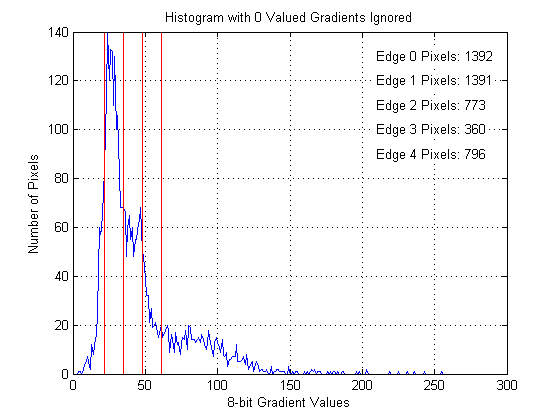
\includegraphics[width=.95\columnwidth]{GradientHistogram}
\label{Flowchart}
\end{figure}

\end{frame}


%%%%%%%%%%%%%%%%%%%%%%%%%%%%%%%%%%%%%%%%%%%%%%%%%%%%%%%%%%%%%%%%%%%%%%%%%%%%%%%
% SYSTEM CONCERNS AND CONSTRAINTS
\begin{frame}[t]{\sc System Concerns and Constraints}

\begin{block}{Multiple View Geometry}
Parallax Disparity and Occlusion Disparity arise from Camera Positions and Scene Content, Structure, and Environmental Conditions
\end{block}

\begin{block}{Information Theory}
Data Set size correlates to amount of Ambiguity; Entropy concerns, also correlates to Data Set size; Major Assumption: PMFs of different views of same scene should be similar
\end{block}


\begin{block}{Feature Detection}
Color Gradients are descriptive of scene objects; Quantization enhances ``Object Detection''; Fast Calculation but Robust against previous concerns
\end{block}

\end{frame}


%%%%%%%%%%%%%%%%%%%%%%%%%%%%%%%%%%%%%%%%%%%%%%%%%%%%%%%%%%%%%%%%%%%%%%%%%%%%%%%
% ALGORITHM FLOWCHART
\begin{frame}[c]{\sc WFMI Algorithm}

\begin{figure}
\centering
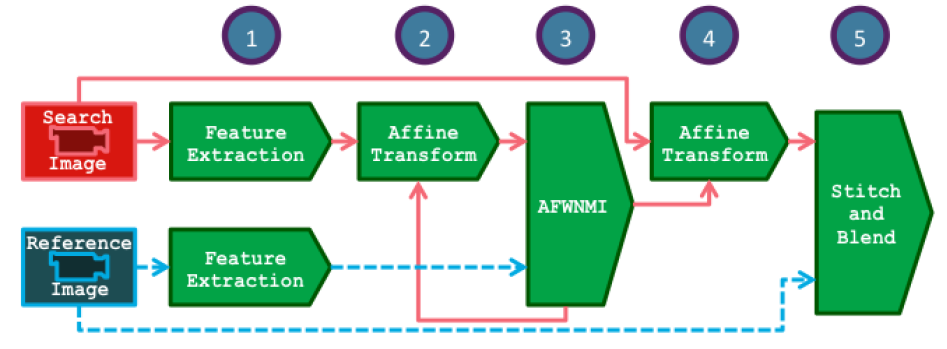
\includegraphics[width=1\columnwidth]{flowchartHorizontal.png}
\label{Flowchart}
\end{figure}

\begin{block}{\footnotesize {\color{yellow}A}bsolute value of {\color{yellow}F}iltered, {\color{yellow}W}eighted, {\color{yellow}N}ormalized {\color{yellow}M}utual {\color{yellow}I}nformation}
Robust to: Low Entropy, Small Overlap, High Amounts of Noise, Large View Disparity
\end{block}


\end{frame}


%%%%%%%%%%%%%%%%%%%%%%%%%%%%%%%%%%%%%%%%%%%%%%%%%%%%%%%%%%%%%%%%%%%%%%%%%%%%%%%
% 0: HIERARCHICAL SEARCH
\begin{frame}[c]{\sc 0: Hierarchical Search}

\only<1>{
\begin{figure}
\centering
\includegraphics[width=.9\columnwidth]{HSearch_001}
\end{figure}
}

\only<2>{
\begin{figure}
\centering
\includegraphics[width=.9\columnwidth]{HSearch_002}
\end{figure}
}

\only<3>{
\begin{figure}
\centering
\includegraphics[width=.9\columnwidth]{HSearch_003}
\end{figure}
}

\only<4>{
\begin{figure}
\centering
\includegraphics[width=.9\columnwidth]{HSearch_004}
\end{figure}
}

\only<5>{
\begin{figure}
\centering
\includegraphics[width=.9\columnwidth]{HSearch_005}
\end{figure}
}


\end{frame}



%%%%%%%%%%%%%%%%%%%%%%%%%%%%%%%%%%%%%%%%%%%%%%%%%%%%%%%%%%%%%%%%%%%%%%%%%%%%%%%
% 1: FEATURE EXTRACTION
\begin{frame}[c]{\sc 1: Feature Extraction}

\only<1>{
\begin{figure}
\centering
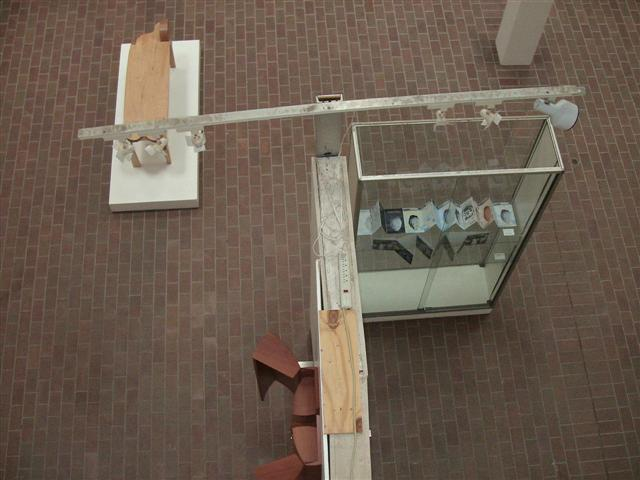
\includegraphics[height=.7\textheight]{AGS4L005}
\caption{Original Image}
\end{figure}
}

\only<2>{
\begin{figure}
\centering
\includegraphics[height=.7\textheight]{AGS4L005gradient}
\caption{Original Image}
\end{figure}
}

\only<3>{
\begin{figure}
\centering
\includegraphics[height=.7\textheight]{AGS4L005edge}
\caption{Original Image}
\end{figure}
}

\end{frame}

%%%%%%%%%%%%%%%%%%%%%%%%%%%%%%%%%%%%%%%%%%%%%%%%%%%%%%%%%%%%%%%%%%%%%%%%%%%%%%%
% 2: AFFINE TRANSFORMATION
\begin{frame}[c]{\sc 2: Affine Transformation}

\only<1>{
\begin{figure}
\centering
\includegraphics[width=.9\columnwidth]{Affine_001}
\end{figure}
}

\only<2>{
\begin{figure}
\centering
\includegraphics[width=.9\columnwidth]{Affine_002}
\end{figure}
}

\end{frame}

%%%%%%%%%%%%%%%%%%%%%%%%%%%%%%%%%%%%%%%%%%%%%%%%%%%%%%%%%%%%%%%%%%%%%%%%%%%%%%%
% 3: AFWNMI
\begin{frame}[c]{\sc 3: AFWNMI Calculation}


\only<1>{
\begin{figure}
\centering
\includegraphics[width=.9\columnwidth]{OverlapFloatRooftop_001}
\end{figure}
}

\only<2>{
\begin{figure}
\centering
\subfigure{\includegraphics[width=.25\columnwidth]{OverlapFloatRooftop_002}}
\subfigure{\includegraphics[width=.05\columnwidth]{Ellipses}}
\subfigure{\includegraphics[width=.25\columnwidth]{OverlapFloatRooftop_003}}
\subfigure{\includegraphics[width=.05\columnwidth]{Ellipses}}
\subfigure{\includegraphics[width=.25\columnwidth]{OverlapFloatRooftop_004}}
\\
\subfigure{\includegraphics[width=.05\columnwidth]{Ellipses}}
\subfigure{\includegraphics[width=.25\columnwidth]{OverlapFloatRooftop_005}}
\subfigure{\includegraphics[width=.05\columnwidth]{Ellipses}}
\\
\subfigure{\includegraphics[width=.25\columnwidth]{OverlapFloatRooftop_006}}
\subfigure{\includegraphics[width=.05\columnwidth]{Ellipses}}
\subfigure{\includegraphics[width=.25\columnwidth]{OverlapFloatRooftop_007}}
\subfigure{\includegraphics[width=.05\columnwidth]{Ellipses}}
\subfigure{\includegraphics[width=.25\columnwidth]{OverlapFloatRooftop_008}}
\end{figure}
}


\only<3>{
\begin{figure}
\centering
\includegraphics[width=.7\columnwidth]{MutualInformation_RooftopShow_001}
\end{figure}
}

\only<4>{
\begin{figure}
\centering
\includegraphics[width=.85\columnwidth]{MutualInformation_RooftopShow_002}
\end{figure}
}

\only<5>{
\begin{figure}
\centering
\includegraphics[width=.85\columnwidth]{WNMImap}
\caption*{WNMI Map}
\end{figure}
}


\only<6>{
\begin{figure}
\centering
\includegraphics[width=.85\columnwidth]{AFWNMImap}
\caption*{AFWNMI Map}
\end{figure}
}


\end{frame}

%%%%%%%%%%%%%%%%%%%%%%%%%%%%%%%%%%%%%%%%%%%%%%%%%%%%%%%%%%%%%%%%%%%%%%%%%%%%%%%
% 4: OPTIMAL AFFINE TRANSFORMATION
\begin{frame}[c]{\sc 4: Optimal Affine Transformation}

\only<1>{
\begin{figure}
\centering
\includegraphics[height=.8\textheight]{OptimalAffine_001}
\end{figure}
}

\only<2>{
\begin{figure}
\centering
\includegraphics[height=.8\textheight]{OptimalAffine_002}
\end{figure}
}


\end{frame}

%%%%%%%%%%%%%%%%%%%%%%%%%%%%%%%%%%%%%%%%%%%%%%%%%%%%%%%%%%%%%%%%%%%%%%%%%%%%%%%
% 5: STITCH AND BLEND
\begin{frame}[c]{\sc 5: Multi-Resolution Spline Blending}

\only<1>{
\begin{figure}
\centering
\includegraphics[height=.7\textheight]{MultiResolutionSpline_001}
\caption{Multiresolution Spline Blending [Burt1983]}
\label{MultiresolutionSpline}
\end{figure}
}

\only<2>{
\begin{figure}
\centering
\includegraphics[height=.7\textheight]{MultiResolutionSpline_002}
\caption{Multiresolution Spline Blending [Burt1983]}
\label{MultiresolutionSpline}
\end{figure}
}

\end{frame}




%%%%%%%%%%%%%%%%%%%%%%%%%%%%%%%%%%%%%%%%%%%%%%%%%%%%%%%%%%%%%%%%%%%%%%%%%%%%%%%
% AFFINE SCENARIOS
\begin{frame}[c]{\sc Affine Scenarios}

\only<1>{
\begin{figure}
\centering
\subfigure{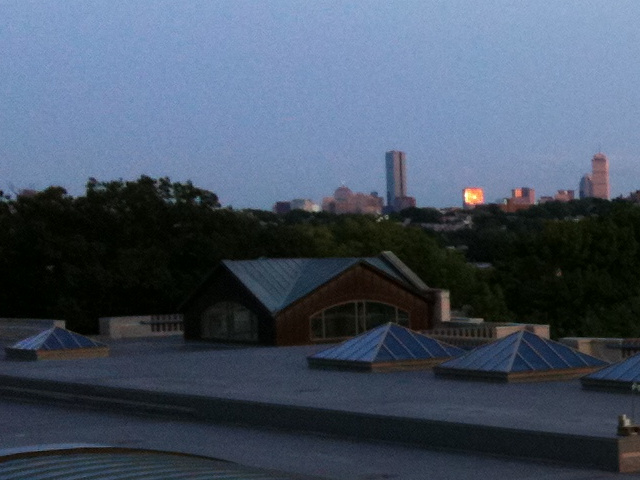
\includegraphics[width=.48\columnwidth]{RooftopL001} \label{RooftopL}}
\subfigure{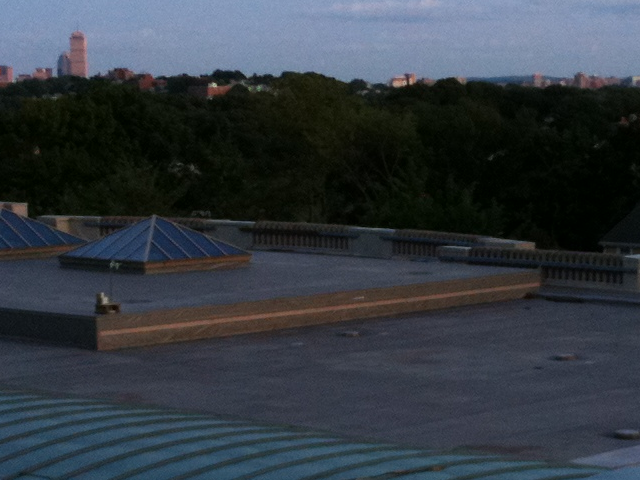
\includegraphics[width=.48\columnwidth]{RooftopR001} \label{RooftopR}}
\caption{Rooftop Scene (a) Left View, (b) Right View}
\label{RooftopImages}
\end{figure}
}


\only<2>{
\begin{figure}
\centering
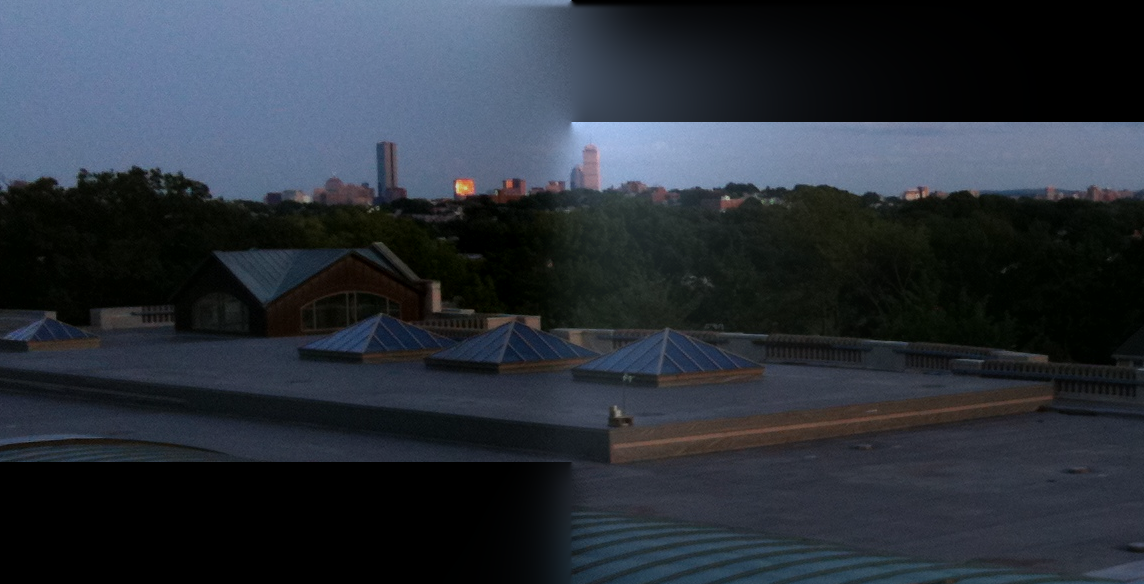
\includegraphics[width=1\columnwidth]{RooftopSP001001}
\caption{Rooftop Views Blended}
\label{RooftopStitched}
\end{figure}
}

\end{frame}



%%%%%%%%%%%%%%%%%%%%%%%%%%%%%%%%%%%%%%%%%%%%%%%%%%%%%%%%%%%%%%%%%%%%%%%%%%%%%%%
% NEAR-AFFINE SCENARIOS
\begin{frame}[c]{\sc Near Affine Scenarios}

\only<1>{
\begin{figure}[!h]
\centering
\subfigure{ 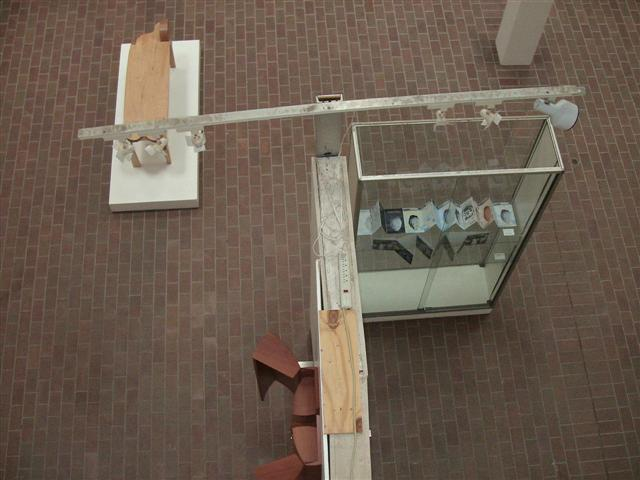
\includegraphics[width=.4\columnwidth]{AGS4L005} \label{ArtGallery4L} }
\subfigure{ 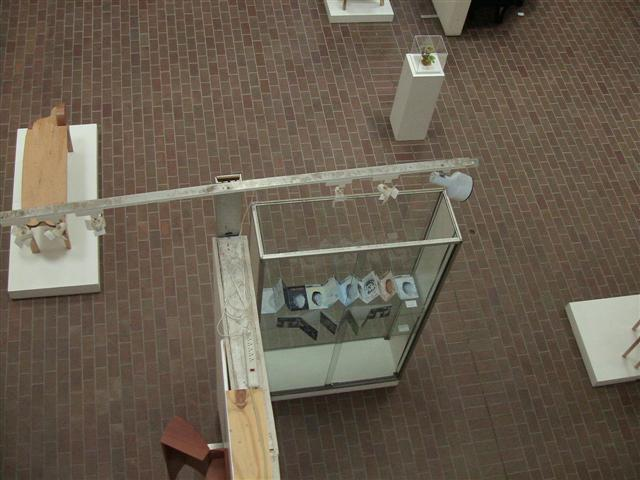
\includegraphics[width=.4\columnwidth]{AGS4R005} \label{ArtGallery4R} }
\caption{Art Gallery 04 Scene (a) Left View, (b) Right View}
\label{ArtGallery4Images}
\end{figure}
}

\only<2>{
\begin{figure}[!h]
\centering
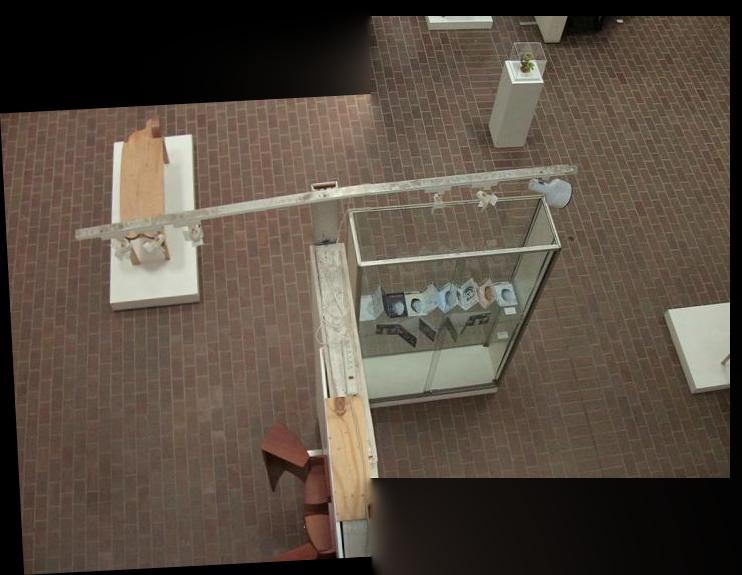
\includegraphics[width=.8\columnwidth]{AGS4SP005005}
\caption{Art Gallery 04 Views Blended}
\label{ArtGallery4Stitched}
\end{figure}
}

\end{frame}


%%%%%%%%%%%%%%%%%%%%%%%%%%%%%%%%%%%%%%%%%%%%%%%%%%%%%%%%%%%%%%%%%%%%%%%%%%%%%%%
% COMPLEX, REAL SCENARIOS
\begin{frame}[c]{\sc Complex, Real Scenarios}

\only<1>{
\begin{figure}
\centering
\subfigure[]{ 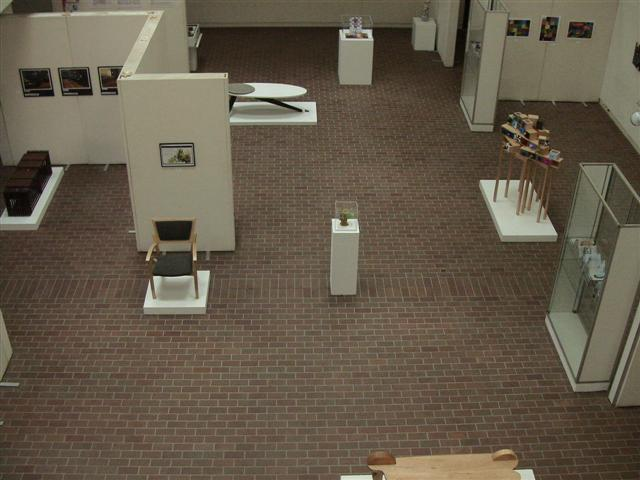
\includegraphics[width=.45\columnwidth]{AGS1L001} \label{ArtGallery1L} }
\subfigure[]{ \includegraphics[width=.45\columnwidth]{AGS1R001} \label{ArtGallery1R} }
\caption{Art Gallery Scene 01 (a) Left View, (b) Right View}
\label{ArtGallery1Images}
\end{figure}
}

\only<2>{
\begin{figure}
\centering
\includegraphics[width=.9\columnwidth]{AGS1SP001001}
\caption{Art Gallery 01 Views Blended}
\label{ArtGallery1Stitched}
\end{figure}
}

\only<3>{
\begin{figure}
\centering
\subfigure[]{ \includegraphics[width=.45\columnwidth]{Lenel010L004} \label{Lenel10L} }
\subfigure[]{ \includegraphics[width=.45\columnwidth]{Lenel010R004} \label{Lenel10R} }
\caption{Lenel Back Lot Scene (a) Left View, (b) Right View}
\label{Lenel10Images}
\end{figure}
}

\only<4>{
\begin{figure}
\centering
\includegraphics[width=1\columnwidth]{Lenel010SP001}
\caption{Lenel Back Lot Views Blended}
\label{Lenel10Stitched}
\end{figure}
}

\end{frame}



%%%%%%%%%%%%%%%%%%%%%%%%%%%%%%%%%%%%%%%%%%%%%%%%%%%%%%%%%%%%%%%%%%%%%%%%%%%%%%%
% CONTRIBUTIONS
\begin{frame}{\sc CONTRIBUTIONS}

\begin{block}{Novel Contribution}
Taking a conceptual understanding of the mathematical concepts and theories of image processing, information theory, and multiple view geometry allowed the development of the novel technique of properly normalizing, weighting, and filtering the mutual information map before the standard method of peak detection.
\end{block}


\vfill

\textsc{Conference Publication:}
\\
{\tiny T. Keane, E. Saber, H. Rhody, A. Savakis, J. Raj, ''Unsupervised automated panorama creation for realistic surveillance scenes through weighted mutual information registration'', \textit{Proceedings of SPIE/IS\&T: Electronic Imaging Symposium}, San Francisco, CA, Jan. 2011}

\vfill

\textsc{Journal Publication:}
\\
{\tiny T. Keane, E. Saber, H. Rhody, A. Savakis, J. Raj, ''Practical image registration concerns overcome by the weighted and filtered mutual information metric'', (Being Submitted for Review) \textit{SPIE/IS\&T: Journal of Electronic Imaging} }
\end{frame}



%%%%%%%%%%%%%%%%%%%%%%%%%%%%%%%%%%%%%%%%%%%%%%%%%%%%%%%%%%%%%%%%%%%%%%%%%%%%%%%
% CONCLUSION
\begin{frame}[c]{\sc Conclusion}
\begin{itemize}
\item Novel Application of Mutual Information
\vfill
\item Realistic Scenes and Practical Concerns
\vfill
\item Novel Approach to Overcome Concerns
\vfill
\item Successful and Conceptually Accurate Estimates
\vfill
\item Not well-worn Research Territory
\vfill
\item Robust to Noise, Entropy, and Overlap Constraints
\vfill
\end{itemize}
\end{frame}


%%%%%%%%%%%%%%%%%%%%%%%%%%%%%%%%%%%%%%%%%%%%%%%%%%%%%%%%%%%%%%%%%%%%%%%%%%%%%%%
% QUESTIONS

\begin{frame}[c]{Questions?}
\centering
{\huge Thank You \vskip .2in I'm Happy to take any Questions:}
\vskip .2in
\begin{itemize}
\item Applied Theory?
\item MATLAB\textsuperscript{\textregistered} Implementation?
\item OpenCV Implementation?
\item Development Process?
\item Results?
\item Future Plans?
\end{itemize}

\end{frame}



%%%%%%%%%%%%%%%%%%%%%%%%%%%%%%%%%%%%%%%%%%%%%%%%%%%%%%%%%%%%%%%%%%%%%%%%%%%%%%%%
%% ACKNOWLEDGEMENTS
%\begin{frame}[c]{Acknowledgments}
%\end{frame}

%%%%%%%%%%%%%%%%%%%%%%%%%%%%%%%%%%%%%%%%%%%%%%%%%%%%%%%%%%%%%%%%%%%%%%%%%%%%%%%
%%%%%%%%%%%%%%%%%%%%%%%%%%%%%%%%%%%%%%%%%%%%%%%%%%%%%%%%%%%%%%%%%%%%%%%%%%%%%%%
% BACKUP SLIDES

\begin{frame}[c]{\sc Appendix}
\begin{center}
\huge APPENDIX
\end{center}
\end{frame}




% Understanding Information Theory
\begin{frame}[c]{\sc Understanding Information Theory}

\vskip -.25in
\begin{figure}
\centering
\subfigure{\includegraphics[width=.50\columnwidth]{InformationTheory3D_L}}
\subfigure{\includegraphics[width=.485\columnwidth]{InformationTheory3D_R}}
\label{infoTheory2}
\end{figure}

\vskip -.25in

\begin{equation}
H(A|B) = H(A,B) - H(B)
\end{equation}

\begin{equation}
H(B|A) = H(A,B) - H(A)
\end{equation}

\end{frame}




% Understanding Information Theory
\begin{frame}[c]{\sc Understanding Information Theory}

\vskip -.25in
\begin{figure}
\centering
\subfigure{\includegraphics[width=.48\columnwidth]{InformationTheory3D}}
\subfigure{\includegraphics[width=.48\columnwidth]{InformationTheoryVenn}}
\label{infoTheory2}
\end{figure}

\begin{equation}
I(A;B) = H(A) + H(B) - H(A,B)
\end{equation}

\end{frame}



% AFFINE AND PROJECTIVE HOMOGRAPHIES
\begin{frame}[c]{\sc Defining Homographies}

\textbf{Affine Homography}:
\begin{equation}
\label{AffineHomographySolve}
\begin{bmatrix}\sfrac{\hat{x}}{1}\\\sfrac{\hat{y}}{1}\\1\end{bmatrix}=\begin{bmatrix}\hat{x}\\\hat{y}\\1\end{bmatrix}=\begin{bmatrix}a_{11}&a_{12}&a_{13}\\a_{21}&a_{22}&a_{23}\\0&0&1\end{bmatrix}\begin{bmatrix}x\\y\\1\end{bmatrix}
\end{equation}

\vfill

\textbf{Projective Homography}:
\begin{equation}
\label{ProjectiveHomographySolve}
\begin{bmatrix}\sfrac{\hat{x}}{\hat{z}}\\\sfrac{\hat{y}}{\hat{z}}\\1\end{bmatrix}=\begin{bmatrix}\hat{x}\\\hat{y}\\\hat{z}\end{bmatrix}=\begin{bmatrix}p_{11}&p_{12}&p_{13}\\p_{21}&p_{22}&p_{23}\\p_{31}&p_{32}&1\end{bmatrix}\begin{bmatrix}x\\y\\1\end{bmatrix}
\end{equation}

\end{frame}



% DIRECT LINEAR TRANSFORMATION
\begin{frame}[t]{\sc Solving for Homographies}

\textbf{Direct Linear Transformation}:

\begin{center}

\vskip -0.15in
\begin{equation}
\label{DLT}
	A=\hat{\bf{x}}_{i} \times H \bf{x}_{i}=0
\end{equation}

\begin{equation}
\label{DLTSVD}
	A=U \Sigma V^{H}
\end{equation}

\begin{equation}
\label{SVD}
	\Sigma = \begin{bmatrix}\sigma_{1}&0&0&0&\cdots&0 \\ 0&\sigma_{2}&0&0&\cdots&0 \\ 0&0&\sigma_{3}&0&\cdots&0 \\ &&&\ddots&& \end{bmatrix}
\end{equation}

\end{center}

\end{frame}


%%%%%%%%%%%%%%%%%%%%%%%%%%%%%%%%%%%%%%%%%%%%%%%%%%%%%%%%%%%%%%%%%%%%%%%%%%%%%%%
% AFFINE SCENARIOS
\begin{frame}[c]{\sc Affine Scenarios}

\only<1>{
\begin{figure}
\centering
\subfigure{\includegraphics[width=.48\columnwidth]{RooftopNoisy191521L001} \label{RooftopNoisy191521L001}}
\subfigure{\includegraphics[width=.48\columnwidth]{RooftopNoisy191521R001} \label{RooftopR}}
\caption{Rooftop Scene 19dB SNR (a) Left View, (b) Right View}
\label{RooftopImages}
\end{figure}
}


\only<2>{
\begin{figure}
\centering
\includegraphics[width=1\columnwidth]{RooftopNoisy191521SP001001}
\caption{Rooftop Views 19dB SNR Blended}
\label{RooftopStitched}
\end{figure}
}



\only<3>{
\begin{figure}
\centering
\includegraphics[width=1\columnwidth]{RooftopNoisy191521001WNMI}
\caption{Rooftop Views 19dB WNMI}
\label{RooftopStitched}
\end{figure}
}

\only<4>{
\begin{figure}
\centering
\includegraphics[width=1\columnwidth]{RooftopNoisy191521001FWNMI}
\caption{Rooftop Views 19dB AFWNMI}
\label{RooftopStitched}
\end{figure}
}

\only<5>{
\begin{figure}
\centering
\subfigure{\includegraphics[width=.48\columnwidth]{StoneWallL001} \label{RooftopNoisy191521L001}}
\subfigure{\includegraphics[width=.48\columnwidth]{StoneWallR001} \label{RooftopR}}
\caption{Stone Wall Scene (a) Left View, (b) Right View}
\label{RooftopImages}
\end{figure}
}


\only<6>{
\begin{figure}
\centering
\includegraphics[width=.8\columnwidth]{StoneWallSP001001}
\caption{Stone Wall Views Blended}
\label{RooftopStitched}
\end{figure}
}

\end{frame}


%%%%%%%%%%%%%%%%%%%%%%%%%%%%%%%%%%%%%%%%%%%%%%%%%%%%%%%%%%%%%%%%%%%%%%%%%%%%%%%
% NEAR-AFFINE SCENARIOS
\begin{frame}[c]{\sc Near Affine Scenarios}

\only<1>{
\begin{figure}[!h]
\centering
\subfigure{ \includegraphics[width=.4\columnwidth]{AGS4L008} \label{ArtGallery4L} }
\subfigure{ \includegraphics[width=.4\columnwidth]{AGS4R008} \label{ArtGallery4R} }
\caption{Art Gallery 04 Scene (a) Left View, (b) Right View}
\label{ArtGallery4Images}
\end{figure}
}

\only<2>{
\begin{figure}[!h]
\centering
\includegraphics[width=.95\columnwidth]{AGS4SP008008}
\caption{Art Gallery 04 Views Blended}
\label{ArtGallery4Stitched}
\end{figure}
}

\end{frame}

%%%%%%%%%%%%%%%%%%%%%%%%%%%%%%%%%%%%%%%%%%%%%%%%%%%%%%%%%%%%%%%%%%%%%%%%%%%%%%%
% COMPLEX, REAL SCENARIOS
\begin{frame}[c]{\sc Complex, Real Scenarios}

\only<1>{
\begin{figure}
\centering
\subfigure[]{ \includegraphics[width=.45\columnwidth]{Lenel005L001} \label{ArtGallery1L} }
\subfigure[]{ \includegraphics[width=.45\columnwidth]{Lenel005R001} \label{ArtGallery1R} }
\caption{Lenel Front Lot Scene (a) Left View, (b) Right View}
\label{ArtGallery1Images}
\end{figure}
}

\only<2>{
\begin{figure}
\centering
\includegraphics[width=.9\columnwidth]{Lenel005SP001001}
\caption{Lenel Front Lot Views Blended}
\label{ArtGallery1Stitched}
\end{figure}
}

\only<3>{
\begin{figure}
\centering
\subfigure[]{ \includegraphics[width=.45\columnwidth]{Lenel005001WNMI} \label{Lenel10L} }
\subfigure[]{ \includegraphics[width=.45\columnwidth]{Lenel005001FWNMI} \label{Lenel10R} }
\caption{Lenel Front Lot Scene (a) WNMI, (b) AFWNMI}
\label{Lenel10Images}
\end{figure}
}


\only<4>{
\begin{figure}
\centering
\subfigure[]{ \includegraphics[width=.45\columnwidth]{Lenel010004WNMI} \label{Lenel10L} }
\subfigure[]{ \includegraphics[width=.45\columnwidth]{Lenel010004FWNMI} \label{Lenel10R} }
\caption{Lenel Back Lot Scene (a) WNMI, (b) AFWNMI}
\label{Lenel10Images}
\end{figure}
}

\end{frame}



% WHY RANDOMNESS
\begin{frame}[c]{\sc Why Randomness?}

\only<1>
{\begin{figure}
\centering
\includegraphics[height=.8\textheight]{PinkBlock}
\label{infoTheory3}
\end{figure}
}

\only<2>
{\begin{figure}
\centering
\includegraphics[height=.8\textheight]{NoiseBlock}
\label{infoTheory3}
\end{figure}
}

\end{frame}




%%%%%%%%%%%%%%%%%%%%%%%%%%%%%%%%%%%%%%%%%%%%%%%%%%%%%%%%%%%%%%%%%%%%%%%%%%%%%%%
% END OF DOCUMENT
%%%%%%%%%%%%%%%%%%%%%%%%%%%%%%%%%%%%%%%%%%%%%%%%%%%%%%%%%%%%%%%%%%%%%%%%%%%%%%%
\end{document}
